\documentclass[11pt,a4paper]{article}
%%%%%%%%%%%%%%%%%%%%%%%%%%%%%%%%%%%%%%%%%%%%%%%%%%%%%%%%
%                      PACKAGES                        %
%%%%%%%%%%%%%%%%%%%%%%%%%%%%%%%%%%%%%%%%%%%%%%%%%%%%%%%%

\usepackage[utf8]{inputenc}
\usepackage{graphicx} % Allows you to insert figures
\usepackage[export]{adjustbox}
\usepackage{booktabs}
\usepackage{amsmath} % Allows you to do equations
\usepackage{helvet}
\usepackage{hyperref}
\renewcommand{\familydefault}{\sfdefault}
\usepackage[a4paper, total={6.5in, 9.5in}]{geometry} % Formats the paper size, orientation, and margins
\linespread{1.1} % about 1.5 spacing in Word
\setlength{\parindent}{0pt} % no paragraph indents
\setlength{\parskip}{1em} % paragraphs separated by one line
\usepackage{listings}
\usepackage{enumitem}
\usepackage{xcolor}
\usepackage{hyperref}
\hypersetup{
	colorlinks=true,
	urlcolor=cyan,
	linktoc=none,
}
\usepackage{fancyhdr}
\pagestyle{fancy}
\fancyhead[L,C,R]{}
\fancyfoot[L]{Blix - AI Photo Editor}
\fancyfoot[C]{}
\fancyfoot[R]{\textbf{\thepage}}
\renewcommand{\headrulewidth}{0pt}
\renewcommand{\footrulewidth}{0.5pt}

\definecolor{codegreen}{rgb}{0,0.6,0}
\definecolor{codegray}{rgb}{0.5,0.5,0.5}
\definecolor{codepurple}{rgb}{0.58,0,0.82}
\definecolor{backcolour}{rgb}{0.95,0.95,0.92}

\lstdefinestyle{mystyle}{
backgroundcolor=\color{backcolour},
commentstyle=\color{codegreen},
keywordstyle=\color{magenta},
numberstyle=\tiny\color{codegray},
stringstyle=\color{codepurple},
basicstyle=\ttfamily\footnotesize,
breakatwhitespace=false,
breaklines=true,
keepspaces=true,
numbers=left,
numbersep=5pt,
showspaces=false,
showstringspaces=false,
showtabs=false,
tabsize=2,
}

\lstset{style=mystyle}
\def\code#1{\texttt{#1}}

%%%%%%%%%%%%%%%%%%%%%%%%%%%%%%%%%%%%%%%%%%%%%%%%%%%%%%%%
%            TITLE PAGE & TABLE OF CONTENTS            %
%%%%%%%%%%%%%%%%%%%%%%%%%%%%%%%%%%%%%%%%%%%%%%%%%%%%%%%%

\begin{document}

\begin{titlepage}
	\centering
    % \includegraphics[width=0.5\textwidth]{your_logo.png}\par\vspace{1cm}
    {\scshape\LARGE Architecture\par}
    \vspace{1.5cm}
    {\huge\bfseries Blix - AI Photo Editor\par}
    \begin{figure}[h]
        \centering % center the image
        
\includegraphics[width=0.5\textwidth]{../pics/blix.png}
    \end{figure}
    \vspace{2.5cm}
    {\Large\itshape The Spanish Inquisition\par}
	\begin{tabular}{|c|c|}
		\hline
		\textbf{Name} 		& \textbf{Student Number} \\
		\hline
		Armand Krynauw		& u04868286  \\
		Jake Mileham		& u21692492  \\
		Dino Gironi			& u21630276  \\
		Karel Olwage		& u21555258  \\
		Francois Combrinck	& u21729752  \\
		\hline
	\end{tabular}
    \vfill
    {\large \today\par}
\end{titlepage}

\tableofcontents
\pagebreak

%%%%%%%%%%%%%%%%%%%%%%%%%%%%%%%%%%%%%%%%%%%%%%%%%%%%%%%%
%                MAIN DOCUMENT CONTENT                 %
%%%%%%%%%%%%%%%%%%%%%%%%%%%%%%%%%%%%%%%%%%%%%%%%%%%%%%%%

\section{Design Strategy}
The architectural design strategy for this software engineering project used two
main approaches: decomposition and design based on quality requirements.

\begin{enumerate}[label*=\arabic*.]
	\item[\textbullet] {\bf Decomposition Strategy}: The decomposition strategy
	involved breaking the system down into individual components or subsystems.
	These components were then designed and implemented independently, and their
	interactions were defined. This approach allowed for a more modular design,
	which made the system easier to understand, maintain, and extend.

	\item[\textbullet] {\bf Requirements Strategy}: The design based on quality
	requirements strategy involved identifying the key quality requirements for
	the system and then designing the system to meet those requirements. This
	approach ensured that the system would be reliable, efficient, secure, and
	usable.
\end{enumerate}

\section{Quality Requirements}

\subsection{Performance}

\begin{enumerate}[label*=\arabic*.]
	\item[\textbullet] {\bf Description}: The application should demonstrate
	efficient speed and responsiveness when editing large images and handling
	multiple projects. Real-time processing of graph-based image operations
	should be seamless and should not cause any delay during editing. The
	application should be able to support the execution of multiple system
	plugins that should not cause any significant performance degradation.

	\item[\textbullet] {\bf Quantification}: The performance requirement will be
	measured by defining specific metrics, such as the maximum size of images
	that can be edited without lag, the duration of time it takes for the
	application to load and display images of various sizes, and the average
	time taken for the application to process a graph-based image operation. The
	application's performance with different numbers of open projects and
	running plugins can also be benchmarked by measuring the percentage of CPU
	and RAM usage and observing performance during peak usage.
\end{enumerate}

\subsection{Security} 
\begin{enumerate}[label*=\arabic*.]
	\item[\textbullet] {\bf Description}: The application must ensure the
	confidentiality, integrity, and availability of user data by protecting
	against unauthorized access, disclosure, modification, or destruction.
	Furthermore, the application and its plugin system must be resilient to
	attacks from third-party entities and malicious users.

	\item[\textbullet] {\bf Quantification}: The application should isolate and
	sandbox plugin code to prevent it from accessing sensitive user information
	and core system functionality.  The application should use encryption for
	sensitive user data both at-rest and in-transit. 
\end{enumerate}

\subsection{Customizability}
\begin{enumerate}[label*=\arabic*.]
	\item[\textbullet] {\bf Description}: The system be extensible and
	customizable to the extent where they can change the theme of the system to
	their liking. Customize application command shortcuts as they see fit and
	change the layout of the system with hot-swappable tiles. The system should
	also allow for custom plugin creation and customization.

	\item[\textbullet] {\bf Quantification}: The system should support a minimum
	of five themes. The system should allow the shortcut customization of base
	system commands and plugin commands. The system should allow users to
	rearrange the the base layout and add custom plugin tiles. The system will
	provide a plugin development API that allows users to create and customize
	their own plugins.
\end{enumerate}

\subsection{Usability} 
\begin{enumerate}[label*=\arabic*.]
	\item[\textbullet] {\bf Description}: The system should be clear and concise
	on how it should be operated. The system must ensure that users can easily
	navigate and use the system without external assistance or unwarranted
	difficulty. The system should provide keyboard navigation for primary parts
	of the system to make powers users more efficient. All functionality must be
	properly documented such that high-end users can easily perform complex
	operations.

	\item[\textbullet] {\bf Quantification}: The percentage of users who are
	able complete a given set of tasks should be above specified threshold. User
	errors rates should be kept to a minimum and users should have and easy and
	pleasant time interacting with the system. 
	
\end{enumerate}

\subsection{Compatibility} 
\begin{enumerate}[label*=\arabic*.]
	\item[\textbullet] {\bf Description}: The application must be compatible
	with major operating systems such as Windows, macOS, and Linux distributions
	such as Ubuntu and Debian. It should support image file formats commonly
	used in the industry such as JPEG, PNG, GIF, BMP, and RAW from popular
	camera brands.

	\item[\textbullet] {\bf Quantification}: The application must be able to run
	without errors on the latest stable versions of the aforementioned operating
	systems. It must be able to import and export image files with the
	aforementioned formats without any data loss or corruption. 
\end{enumerate}

\pagebreak

\section{Architectural Design \& Patterns}
Four main architectural patterns where identified to decompose the base system
into components and subsystems.

\begin{figure}[ht]
	\centering
	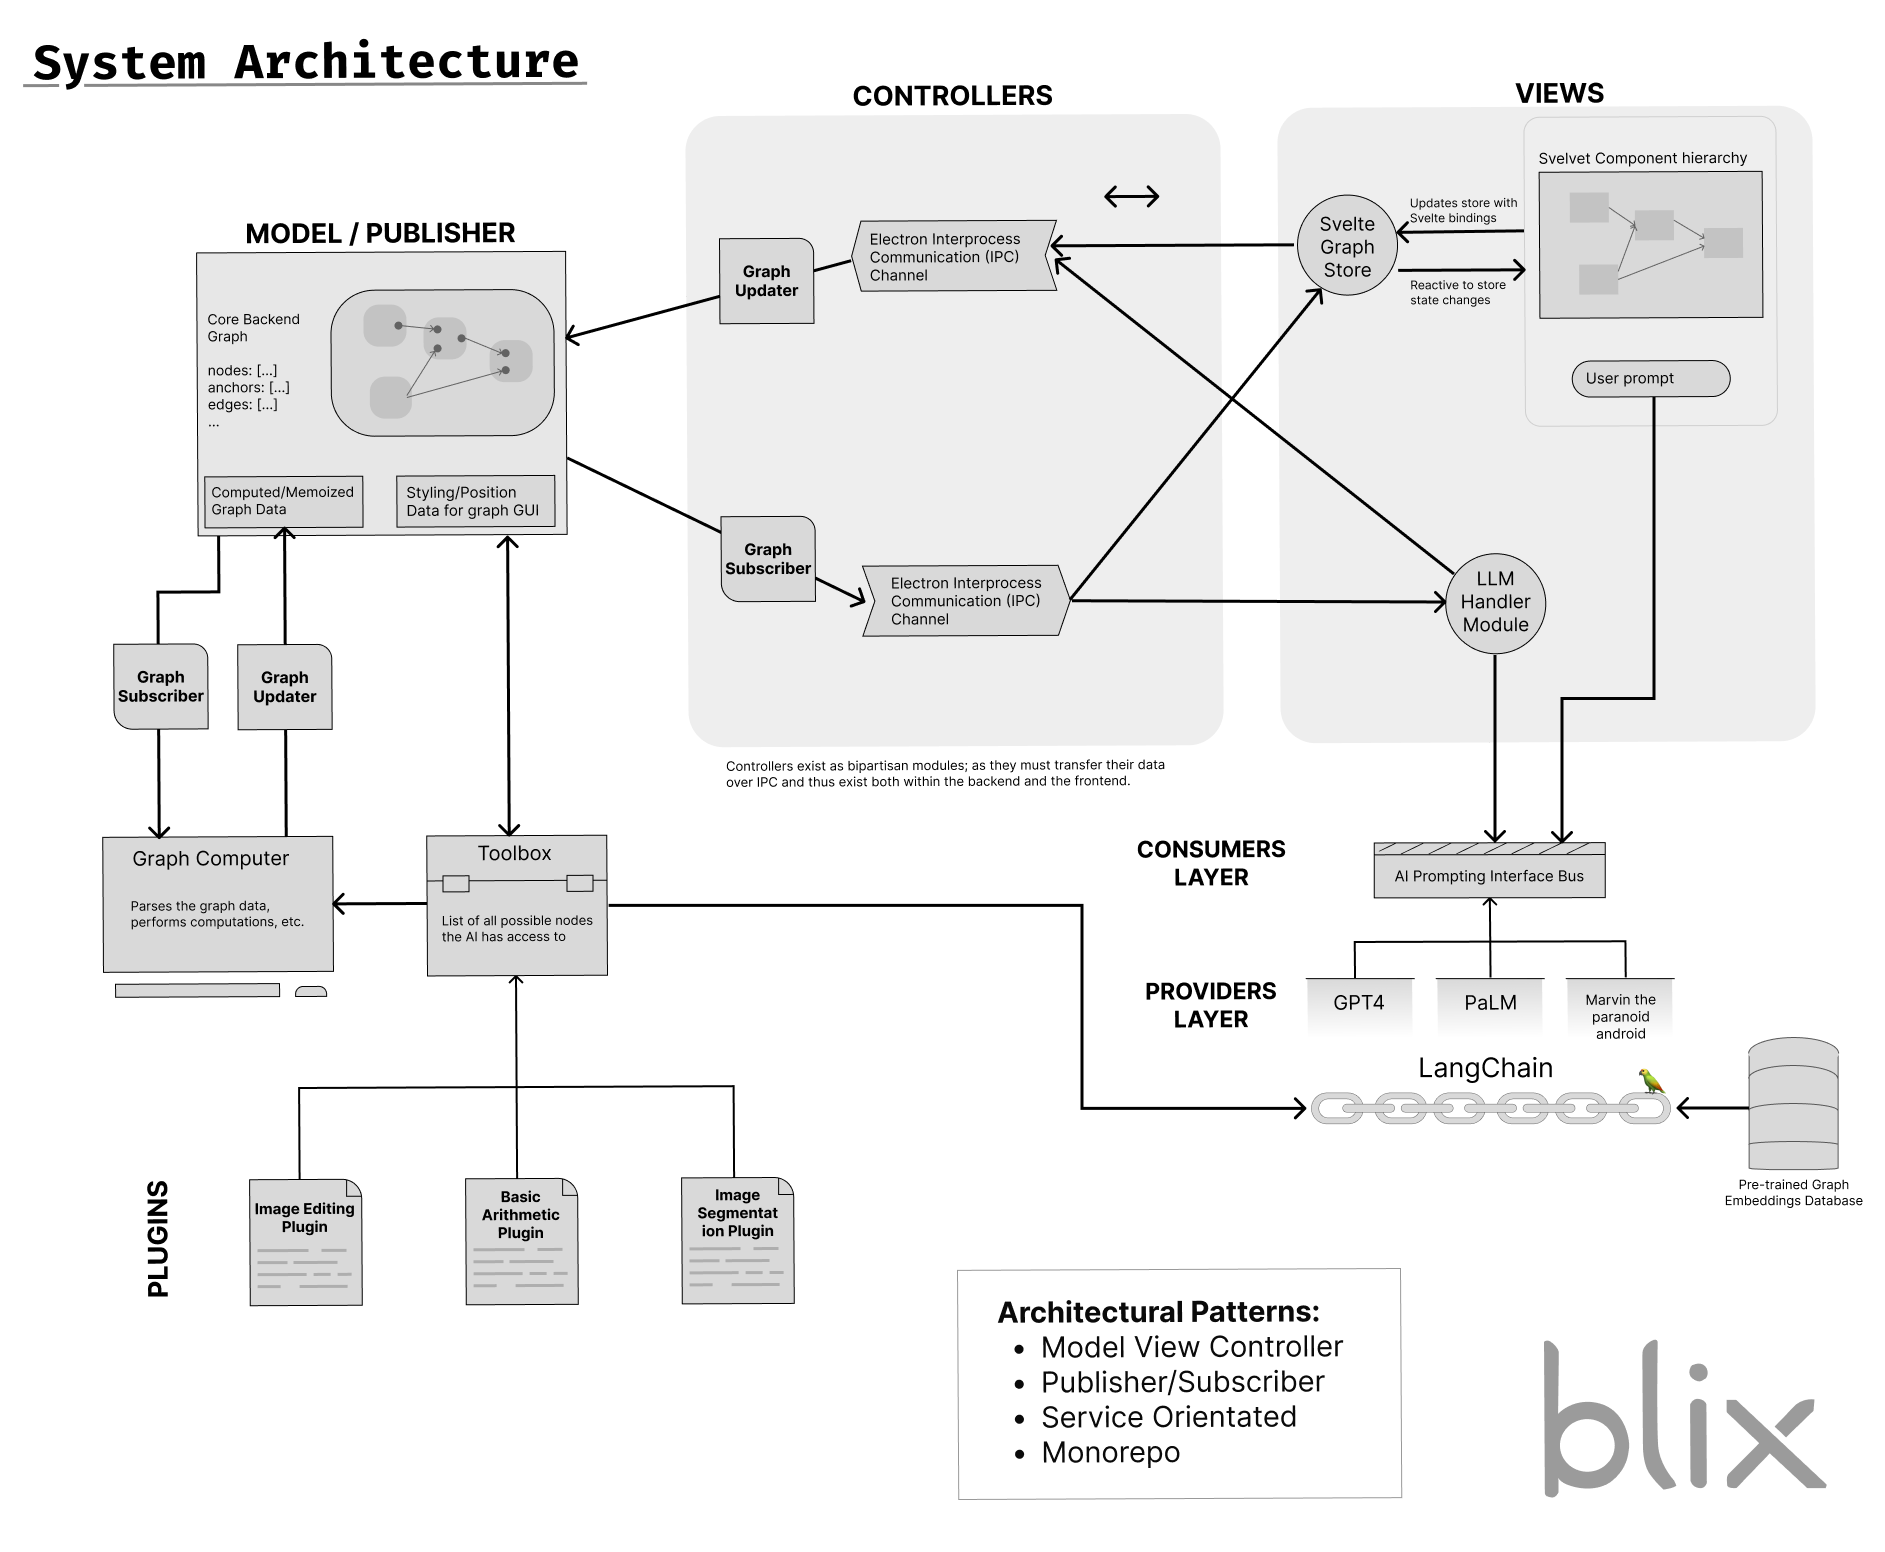
\includegraphics[width=1\textwidth,height=\textheight,keepaspectratio,rotate=0,origin=c]{../diagramPng/SystemArchitecture.png}
\end{figure}

\subsection{Model-View-Controller (MVC)}
The MVC pattern was chosen in order to create clear distinction between the user
interface, business logic and system data. This trinity-based setup enables
separation of concerns and allows for the system to be easily extended and
maintained. Each of the three components play their parts as follows:
\begin{enumerate}[label*=\arabic*.]
	\item[\textbullet] {\bf Model}: The 'model' in our system is the core
	backend graph running on the Node.js server within the Electron application.
	This represents the core state of the system, and is the central source of
	truth for all other views in the system. In a sense, it acts as a central
	database which all other 'services' utilize.
	\item[\textbullet] {\bf Views}: Our system consists of multiple views which
	all derive representations from the core graph {\it model}. Some examples of
	views in the system include the frontend {\it Svelvet} graph which the user
	interacts with, as well as the text-based (e.g. JSON) model which is passed
	to the LLM AI assistant. When changes take place within the core graph,
	these views are automatically updated to reflect them.
	\item[\textbullet] {\bf Controllers}: These are the 'middle-men' between
	each view, and the core graph. As our system is an Electron application, the
	frontend views must be able to communicate with the core graph over
	Electron's IPC ({\it Interprocess Communication}) protocol.

	When changes to local view state take place (e.g. If the user were to add a
	new node to the frontend graph), the controllers are responsible for
	instructing the core backend graph that these changes have taken place. Then
	after the core graph has applied these changes in a manner that is
	consistent (forms a valid directed compute graph), all subscriber views are
	notified of the changes and are updated accordingly.
\end{enumerate}


\subsection{Publish-Subscribe}
Our implementation layers the Publish-Subscribe architectural pattern on top of
the MVC pattern to endow the system with multiple-reactivity. The PubSub
architecture allows one central source of information to be propagated to a
multitude of subscribers, in our case the core graph and each of its views
respectively. PubSub is a highly effective pattern as it abstracts the notion of
state propagation into a composable set of participant modules which can be
easily added/removed from the system. This helps us future-proof the application
and allows for scalability as the system grows.

As an example, let's say down the line we wanted to add a command line utility
to compute a given graph without needing the user interface to be loaded; In
such a situation we could easily disable the UI graph subscriber, and add
alongside a 'command line utility' subscriber, which still communicates with the
core graph, but does so entirely through the standard input/output streams of
the command line.

Thus by using this architecture we have effectively made core parts of the
system 'hot-swappable'.

\subsection{Service-Oriented}
The Service-Oriented architectural pattern exists within an essential aspect of our system, the AI LLM assistant.
This pattern enables modularity, flexibility, and extensibility by defining the system's components as a collection of distinct services.
Here we treat each LLM model as a separate service, which can be added, removed, or swapped out with another model.

Models that may be supported as 'services' include GPT-3, GPT-4, PaLM, etc.
Each of these models can subscribe to the core graph and make updates to it.
Moreover, by leveraging the power of LangChain using a custom pre-trained vector database of graph {\it word2vec} embeddings,
the Service-Oriented architecture helps us to create a comprehensive and efficient system for managing these models and enhancing their capabilities with domain-specific knowledge.

This allows for seamless exchanging of information among the services, as well as smooth updating and enhancement of the system when new AI models become available or when updates to existing models are released.
Consequently, the Service-Oriented architecture maximizes the potential of our AI-driven system by promoting modularity, interoperability, and the rapid development of new features and capabilities.


% \subsection{Client-Server}
% The Large Language Model AI assistant is a significant part of the system which
% we are building, and at the time of writing all major LLMs (which provide the
% sufficient level of intelligence that we are looking for) are hosted on the
% cloud. As our app is hosted natively on this users machine, this means we must
% also enable remote communication to the respective LLM API's.

% From this perspective, the Blix application exists as a client to the LLM API
% server, and must be able to perform remote HTTP requests as such. Google has
% recently announced the release of their PaLM models as open source, however, and
% so we are currently investigating the possibility of hosting the LLM locally on
% the users machine. In such a situation the client-server architecture would
% still apply, except that the server 'LLM API' would be hosted locally on the
% users machine, and all communication would be done over the loopback interface.


\section{Constraints}

No special constraints or limitations have been identified or explicitly
communicated by the client.

\section{Technology Choices}

\subsection{Svelte}
Svelte is an open-source JavaScript framework for building user interfaces. It
is designed to be highly efficient and focused on delivering optimal performance
by shifting the work from the runtime to the build process. One of the key
visions of Blix is to provide a fast and responsive user interface with
lightning fast reactivity. Additionally due to the large scope of the project,
it is important to ensure that the system is as lightweight as possible. Svelte
is the perfect choice for this as it compiles the application into highly
performant JavaScript, instead of simulating a virtual DOM for performing
reactive page updates.

\textbf{Pros:}
\begin{enumerate}[label*=\arabic*.]
	\item[\textbullet] Fast and responsive user interface with lightning fast
	reactivity. 
	\item[\textbullet] Svelte is a highly scalable framework that allows for the
	creation of large scale applications.
	\item[\textbullet] Reusability of components shortens development time.
\end{enumerate}


\textbf{Cons:}
\begin{enumerate}[label*=\arabic*.]
	\item[\textbullet] Svelte is a relatively new framework and as such has a
	smaller community than other frameworks such as React and Vue.
	\item[\textbullet] Svelte has a smaller ecosystem than other frameworks such
	as React and Vue.
	\item[\textbullet] Svelte is lacking in stability as it is still a
	relatively new framework.
\end{enumerate}

\subsection{Tailwind CSS}
Tailwind CSS is an utility-first CSS framework that provides a set of
pre-designed, low-level utility classes. Tailwind CSS focuses on providing a
comprehensive set of utility classes that you can combine to build custom user
interfaces. Tailwind CSS is the perfect choice for Blix as it allows for the
creation of a custom user interface that is unique to Blix. Additionally,
Tailwind CSS is highly scalable and allows for the creation of large scale
applications.

\textbf{Pros:}
\begin{enumerate}[label*=\arabic*.]
	\item[\textbullet] Tailwind CSS is a scalable framework that allows for the
	creation of large scale applications.
	\item[\textbullet] Tailwind CSS is a customizable framework that allows for
	the creation of a custom user interface that is unique to Blix.
	\item[\textbullet] Tailwind CSS is a responsive framework that allows for
	the creation of a responsive user interface.
\end{enumerate}

\textbf{Cons:}
\begin{enumerate}[label*=\arabic*.]
	\item[\textbullet] The class names can make the HTML markup harder to read
	and maintain, especially for larger projects.
	\item[\textbullet] Tailwind CSS generates a large CSS file due to the
	extensive collection of utility classes. 
	\item[\textbullet] The class names can make the markup harder to read and
	maintain, especially for larger projects.
\end{enumerate}

\subsection{Electron}

Electron allows developers to build cross-platform desktop applications using
web technologies such as HTML, CSS, and JavaScript. Electron allows developers
to locally host a web application within a desktop application. This allows for
the creation of a desktop application that is highly scalable and can be easily
ported to other platforms.
\textbf{Pros:}

\begin{enumerate}[label*=\arabic*.]
	\item[\textbullet] Highly scalable framework that allows for the creation of
	large scale applications.
	\item[\textbullet] Electron provides a comprehensive set of APIs that allows
	for the creation of a desktop application that is unique to Blix.
	\item[\textbullet] Allows code reuse as the same codebase can be used to
	create a desktop application and a web application.
	\item[\textbullet] Leverages the power of Node.js modules to provide 
\end{enumerate}
\pagebreak
\textbf{Cons:}

\begin{enumerate}[label*=\arabic*.]
	\item[\textbullet] Electron generates a large executable file due to the
	extensive collection of APIs.
	\item[\textbullet] High memory usage due to the extensive collection of
	APIs.
	\item[\textbullet] Dependent on chromium browser updates.
\end{enumerate}


\subsection{Firebase}

Firebase is a mobile and web application development platform developed by
Firebase, Inc. in 2011, then acquired by Google in 2014. Firebase provides a
comprehensive set of APIs that allows developers to build, manage, and deploy
applications. Firebase is the perfect choice for Blix as it provides a
comprehensive set of APIs that allows for the creation of a highly scalable
application.

\textbf{Pros:}
\begin{enumerate}[label*=\arabic*.]
	\item[\textbullet] Real time database that allows for the creation of a
	highly scalable application.
	\item[\textbullet] Cloud storage that allows for efficient data storage and
	retrieval.
	\item[\textbullet] Quick and easy authentication that allows for the
	creation of a secure application.
\end{enumerate}

\textbf{Cons:}
\begin{enumerate}[label*=\arabic*.]
	\item[\textbullet] Lack of flexibility as Firebase is a closed source
	platform.
	\item[\textbullet] Limited server side logic as Firebase is a closed source
	platform.
	\item[\textbullet] Scalability and latency considerations is an external
	service.
\end{enumerate}


\subsection{LangChain}

Langchain is a new framework built around llm that allows developers to build
applications that capitalize on the knowledge base and computational power of 
llm's such as gpt-3 by provided the llm's with specialized knowledge on the 
applications domain. Langchain is usefull for Blix as it allows for the manipulation
of the graph and photos using natural language and llms. 

\textbf{Pros:}
\begin{enumerate}[label*=\arabic*.]
	\item[\textbullet] Local storage of context and knowledge base.
	\item[\textbullet] Chaining of llm's to exploit different llm's strengths.
	\item[\textbullet] Allows for the creation of a highly scalable application.
	\item[\textbullet] Flexibility as Langchain is an open source platform.
\end{enumerate}

\textbf{Cons:}
\begin{enumerate}[label*=\arabic*.]
	\item[\textbullet] Lack of solid documentation as Langchain is a new framework.
	\item[\textbullet] Generally requires more requests to llm's to achieve the desired result.
	\item[\textbullet] Lack of integrations for a typescript environment.
\end{enumerate}
\end{document}